\chapter{Information Theoretic and Language Model based Term Extraction using Pointwise Mutual Information}
\chaptermark{Term Extraction using Pointwise Mutual Information}
\label{chap:lmpmi}

This chapter\footnote{Part of the search presented in this thesis has been previously published in \cite{lilingexperttechreport,lilingexpertworkshop}} describes the first main contribution of the thesis, i.e. a novel term extraction technique we have developed based on information theoretic Pointwise Mutual Information (PMI) and language model probabilities. We dub the method $PMI_{LM}$.

The rest of this chapter will first introduce (i) the description of our new monolingual extraction technique, (ii) an intrinsic evaluation of our extraction method against a gold standard terminology, (iii) an extrinsic evaluation of the term extraction in an information retrieval query task and (iv) the bilingual extension of our term extractor based on phrase alignments, iv) an extrinsic evaluation of the automatically extracted bilingual terms on two diverse machine translation tasks.

We show that our monolingual $PMI_{LM}$ term extractor has comparable results with state-of-art term extraction systems in both intrinsic and extrinsic evaluations. Our results of adding terms extracted using the bilingual extension of the $PMI_{LM}$ model agree with previous studies in using additional lexical information in statistical machine translation.

\section{Pointwise Mutual Information}

The Pointwise Mutual Information (PMI) measures the association between two discrete random variables by dividing their joint probability\footnote{i.e. probability of their coincidence} by their individual probabilities\footnote{assuming statistical independence between the variables}. Mathematically,
\vspace{-2mm}
\begin{equation}
\begin{split}
PMI(x,y) & =\log { \frac { p(x,y) }{ p(x)p(y) }  } \\
         & =\log { p(x,y) } -\log { p(x) } -\log { p(y) } 
\end{split}
\end{equation}
\vspace{-2mm}
Applying the chain rule on the PMI equation, we can measure the association between more than two discrete random variables\footnote{See prove on https://en.wikipedia.org/wiki/Pointwise\_mutual\_information\#Chain-rule\_for\_pmi} as such:
\vspace{-2mm}
\begin{equation}
\begin{split}
PMI(xy,z) & =\log { \frac { p(xy,z) }{ p(xy)p(z) }  } \\
& =\log { p(xy,z) } -\log { p(xy) } -\log { p(z) } \\ 
& = PMI(y,z)+PMI(z,y|x) 
\end{split}
\end{equation}
\vspace{-2mm}
In the context of terminology extraction, we can measure the collocation coherence between two words by measuring their PMI \cite{bouma2009normalized,eichler2010dfki}.  For example, to measure the PMI value of the phrase `floating point' 
\vspace{-2mm}
\begin{equation}
\begin{split}
PMI(floating \ point) & =\log { \frac { p(floating \ point) }{ p(floating)p(point) }  } \\
& =\log { p(floating \ point) } -\log { p(floating) } -\log { p(point) } 
\end{split}
\end{equation}
\vspace{-2mm}
where $p(floating,point)$ is the probability of the phrase `\textit{floating point}' divided by the probability of the word `\textit{floating}` and `\textit{point}` occurring individually.

Extending the PMI application to natural text with the chain rule, we can easily find the PMI phrases with more than two words. E.g. for the phrase `\textit{floating point arithmetic}', we can recursively sum the PMI scores of the phrase and the sub-phrases and its sub-phrase.
\vspace{-2mm}
\begin{equation}
\begin{split}
PMI(floating \ point,arithmetic) 
& = \log { p(floating \ point \ arthimetic) } \\
& \quad- \log { p(floating \ point) } -\log { p(arthimetic) } \\ 
% & = pmi(point,arithmetic) + pmi(arithmetic,point|floating) 
\end{split}
\end{equation}

\section{Term Extraction Using Language Model Pointwise Mutual Information}
The calculation of word probabilities and PMI described so far
%in our brief term extraction survey in Chapter 2 
is based on raw counts of a word or term (in Chapter 3 Section 2.5.1). 
$N$-gram language models, that are also based on counts, have developed and applied to other NLP applications such as speech processing and machine translation \citep[e.g.][]{smorgasbord,kirchhoff2005improved,schwenk2012large,lembersky2012adapting,chelba2012distributed}.

A major advantage of using a language model is the possibility of accounting for unknown words using interpolation and smoothing techniques \citep{chen1996empirical,chelba2010}. By using a language model, we avoid the need to optimize n-gram counting when implementing the term extraction algorithm, especially when very fast implementations of language models already exists \citep{kenlm}.

Instead of the using phrasal and word probabilities to compute the PMI score of a term, 

\begin{equation}
PMI(term) = \log { p(w_1,...,w_n) } -\log { p(w_1,...w_{n-1}) } -\log { p(w_n) } 
\end{equation}

we can use a backoff language model as follows:

\begin{equation}
\begin{split}
{ PMI }_{ LM }(term) & = \frac { P_{LM}({ w }_{ 1 },...,{ w }_{ n }) }{ P_{LM}({ w }_{ 1 },...{ ,w }_{ n-1 })P_{LM}({ w }_{ n }) }   \\
& = P_{LM}({ w }_{ 1 },...,{ w }_{ n }) -  P_{LM}({ w }_{ 1 },...,{ w }_{ n-1 }) - P_{LM}({ w }_{ n })
\end{split}
\end{equation}

where a $term$ is made up of words ${ w }_{ 1 },...,{ w }_{ n }$ and $P_{LM}(w)$ is the language model probability provided by a pre-trained language model that approximates to $\log{p(w)}$.

\iffalse
%where ${ PMI }_{ LM }(t)$ is the Pointwise Mutual Information (PMI) score based on language model termhood probability of a term $t$ and $n$ is the total no. of possible $n$-grams (unigrams, bigrams and trigrams) and ${ PMI }_{ LM }({ ngram }_{ i })$ refers to the language model score of the word and its following word. 

%The brevity normalization $1/n$ does not favour a longer term compared to the C-value \citep{frantzi1998c} and the inner context probabilities have either been handled by the $n$-gram model during training or the backoff probability. When an unknown word exists in the term, it uses the backoff probability with the contextual probability of an unknown word occurring in the $w_{i-1}$ and $w_{i-2}$ context.

For example, for the phrase \emph{`floating point arithmetic'} and \emph{`floating point routine'}, we assume that the word \emph{`arithmetic'} is not found in the language model training corpus. Hence the other probabilities were calculated by the language model as follows:

\begin{equation}
{ PMI }_{ LM }('floating \ point \ arithmetic')=1/3! \ *
\left (
\begin{matrix} 
{ P }_{ LM }('floating \ point \ routine') \\
- { P }_{ LM }('floating \ point')
- { P }_{ LM }('point \ routine')
\end{matrix} 
\right )  
\end{equation}

\begin{equation}
{ PMI }_{ LM }('floating \ point \ <UNK>')=1/3! \ *
\left (
\begin{matrix} 
{ P }_{ LM }('floating \ point \ UNK') \\
- { P }_{ LM }('floating \ point')
- { P }_{ LM }('point \ routine')
\end{matrix} 
\right ) 
\end{equation}

\begin{equation}
{ PMI }_{ LM }('floating \ point')=
\begin{matrix} 
{ P }_{ LM }('floating \ point') \\
-({ P }_{ LM }('floating')+{ P }_{ LM }('point'))
\end{matrix} 
\end{equation}

\begin{equation}
{ PMI }_{ LM }('point \ arithmetic')=
\begin{matrix} 
{ P }_{ LM }('point \ UNK') \\
-({ P }_{ LM }('point')+{ P }_{ LM }('UNK')) 
\end{matrix} 
\end{equation}

where ${ P }_{ LM }$ is the language model scores retrieved from the pre-trained trigram language model.
\fi

Similar to the C-value and NC-value \citep{frantzi1998c}, our approach is limited to multi-word expressions. Our approach is (i) a more flexible approach than C-value that allows querying a smoothed language model to retrieve probabilities and (ii) relies on the backoff probabilities that have the ability to score unknown words. The traditional C-value would count co-occurrence instances without smoothed counts and would not handle unknown words. 

%We note that for the single term PMI, we force a PMI value to be isolated from the context where the term occurs. If we use the previous context word before the term, we could get a similar candidate re-ranking as from the NC-value. We did not experiment with the context because we note that finding the correct weights for the C-value and NC-value's cumulative context weight (CCW) should not be as trivial as assigning static 0.2 and 0.8 coefficients in the NC-value calculations. 
%From here on, we refer to our term extraction metric described above as the Language-model PMI ($PMI_{LM}$).

\newpage
\section{Evaluating $PMI_{LM}$ against a Gold Standard}

Intrinsically, we will evaluate the $PMI_{LM}$ against a gold standard terminology in the Biomedical domain. \cite{gurulingappa18empirical} created the \textit{Disease Names and Adverse Effect} (DNAE) corpus with manually annotated medical terms and empirically evaluated a rule-based term extractor, ProMiner, \citep{Hanisch2005}. The ProMiner system uses a pre-processed hand-crafted synonym dictionary to identify potential name occurrences in the biomedical text and associate protein and gene database identifiers with the detected matches. 

\cite{Hanisch2005} considered a subset of the medical terms of the following medical term databases that occurred in the DNAE corpus as the positive examples of the terms that a term extractor should extract. We use the same subset to compare our approach with \cite{Hanisch2005}.

\begin{table}[H]
\centering
    \begin{tabular}{llccc}
    \textbf{System}      & \textbf{Methodology}                 & \textbf{Precision} & \textbf{Recall} &\textbf{ F-score} \\ \hline
    ProMiner    & Unsupervised Rule-based                & \textbf{0.18}      & 0.76   & \textbf{0.29}    \\
    $PMI_{LM}$ (global)     & Unsupervised Probabilistic             & 0.17      &\textbf{ 0.89 }  & \textbf{0.29}    \\ 
    $PMI_{LM}$ (local)     & Unsupervised Probabilistic             & 0.15      &\textbf{ 0.83 }  & 0.25   \\ \hline
    BiOpeNER    & Supervised Off-the-shelf               & \textbf{0.55}      & 0.44   & 0.49    \\
    LM-PMI Linear  & Supervised using Probabilistic Feature & 0.51      & 0.56   & 0.53    \\
    LM-PMI XGBoost  & Supervised using Probabilistic Feature & 0.53      & \textbf{0.58}   & \textbf{0.55 }   \\
    \end{tabular}
\caption{Comparison of $PMI_{LM}$ against State-of-Art Term Extractors}
\label{table:pmllmbiomed}
\end{table}

To directly compare our unsupervised approach (i.e. without the use of the mention annotations from the corpus) against the rule-based ProMiner, we use the $PMI_{LM}$ in two different settings\footnote{Note that the $PMI_{LM}$ approach is limited to multi-word expressions, i.e. ngram orders of two and above. We fall back to the language model probabilities when computing the unigram term scores.} (i) we extracted all possible unigrams to fivegrams from each sentence and filter the top 1200 unique terms weighted by the their 5-gram $PMI_{LM}$ and we search through all documents to label the mentions of these terms, i.e. $PMI_{LM}$ (global) and (ii) we extracted the top 2 unigrams to fivegrams from each sentence and we considered them as the biomedical term that our system identified, i.e. $PMI_{LM}$ (local). Using these two settings, we extracted the terms from the full DNAE corpus and evaluate against the manually annotated terms.

\begin{figure}[!htb]
\centering
	\hspace{-2em}%
	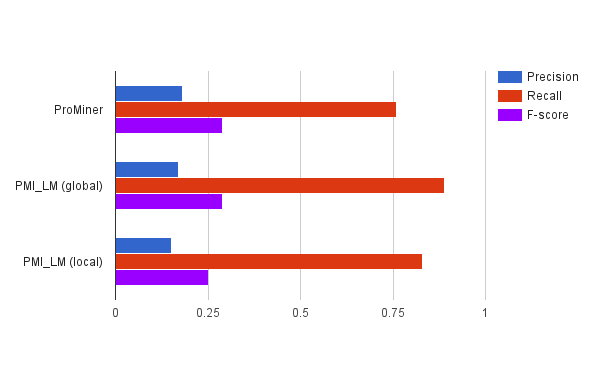
\includegraphics[width=17cm]{unsuper-intrinsic.png} \\[-1em]
	\caption{Precision, Recall and F-score of Unsupervised Term Extraction of $PMI_{LM}$ and ProMiner on the DNAE Corpus}
	\label{fig-unsuper-intrinsic}
\end{figure}

\begin{figure}[!htb]
\centering
	\hspace{-2em}%
	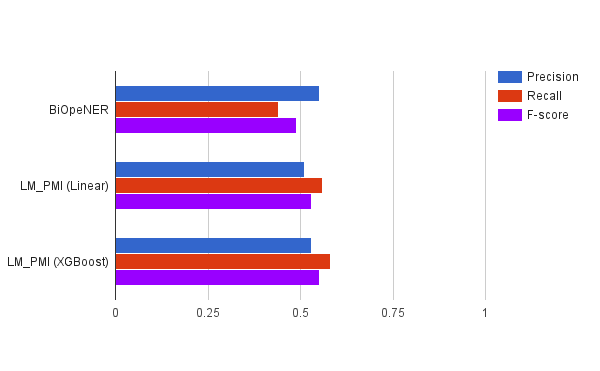
\includegraphics[width=17cm]{super-intrinsic.png} \\[-1em]
	\caption{Precision, Recall and F-score of Supervised Term Extraction of $PMI_{LM}$ and ProMiner on the DNAE Corpus}
	\label{fig-unsuper-intrinsic}
\end{figure}


In the unsupervised scenario, our $PMI_{LM}$ (global) term extractor achieved a similar F-score (0.29) to ProMiner , however our $PMI_{LM}$ (local) system underperformed (F-score=0.25) as compared to ProMiner due to poor precision. This is indirectly caused by the heuristic we impose when extracting the top 2 $PMI_{LM}$ scoring terms per sentence, when in fact there can be 0 or 1 or more than 2 terms within the sentence. 
%In this respect, it reinforces the assumption that salient terms should span across the documents globally and not to every sentence or document. 
On the plus side, we have achieved better recall in both local and global settings at 0.89 and 0.83 respectively as compared to ProMiner that has a recall rate of 0.76.

In a supervised scenario, we use our $PMI_{LM}$ score of all possible ngrams as a sparse feature set to train a linear classifier\footnote{Using the default linear logistic classifier from Scikit-learn\citep{Pedregosa2011}} and an XGBoost ensemble classifier\footnote{Using {\tt hammer.py} wrapper script from \citep{bechara-EtAl:2016:SemEval}. Note that we further slice the 90\% training set to 80\% train and 10\% development to tune the system at every fold for our ensemble system} \citep{chenxgboost} to identify the terms from the manually annotated DNAE corpus. We randomly split the sentences with and 90\% train and 10\% test set and report the harmonic cross-validation precision, recall and F-scores in Table 3.2. We compare our results against the BiOpeNER \citep{biopener} system that also reported harmonic cross-validation scores. 

Although our system did not achieve the state-of-art precision scores that BiOpeNER had, both the linear logistic and ensemble classifier performed better on the recall scores and F-scores. The BiOpeNER system achieved 0.55 precision, 0.44 recall and 0.49 F-score whereas our best setup with the XGBoost achieved 0.53 precision, 0.58 recall and 0.55 F-score.

\section{Evaluating $PMI_{LM}$ in Information Retrieval}

As an extrinsic evaluation, we test the $PMI_{LM}$ term extraction approach on the food domain corpus (WikiFood) that was built for an ontology induction task at SemEval-2015. The corpus contains 869 food terms and the relevant Wikipedia articles that contain these terms. Of those terms 752 terms are multi-words and from the 752 multi-words, we extracted 42,851 sentences (1,207,677 tokens) that contains the multi-word terms. 
%We expect only 1 correct term to be extracted per sentence. 

To access the probabilities for calculating ${ PMI }_{ LM }$, we trained a 5-gram language model on the corpus and we evaluate the ${ PMI }_{ LM }$ accuracy against the traditional C-value score in extracting terms from the corpus. 

We extract the top five term candidates each using ${ PMI }_{ LM }$ and C-value to match against the 1 correct term per sentence. We evaluate the metrics by calculating the accuracy of the top ranked term candidates for each sentence and matching them against the correct term for that sentence. Since the experimental task is structured more like an information retrieval task of candidate ranking, we use the mean reciprocal rank (MRR) to evaluate the ranking efficiency of the term extraction metrics. The mean reciprocal rank is calculated by averaging the ranks of the retrieved candidates against all possible candidates.

\begin{table*}[ht!]
\centering
    \begin{tabular}{l|cc|c}
    ~       & Accuracy (\textit{Top1}) & Accuracy (\textit{Top5}) & MRR   \\ \hline
    \textbf{$PMI_{LM}$}   & \textbf{28.29}           & \textbf{45.18}           & \textbf{1.632} \\
    C-Value & 23.26           & 32.26           & 2.263 \\
    \end{tabular}
\caption{Accuracy and Mean Reciprocal Rank for Term Extraction for WikiFood}
\label{table:pmilmeval}
\end{table*}

Table \ref{table:pmilmeval} presents the results of the experiment on term extraction for the WikiFood Corpus. The $PMI_{LM}$ metric clearly scores better in terms of accuracy to rank the correct term candidate in the top position with a mean rank of 1.63 and an accuracy of 0.28 compared to the C-value’s mean rank of 2.26 and an accuracy of 0.23.

\begin{table*}[ht!]
\centering
    \begin{tabular}{ll|ll}
     \textbf{C-Value}                  & ~      & $PMI_{LM}$                      & ~      \\ \hline
    Bull’s-Eye Barbecue Sauce & -6.491 & Burger King              & -3.269 \\
    Al Steak Sauce            & -7.078 & Bull’s-Eye Barbecue Sauce & -4.909 \\
    Kraft products            & -7.397 & A1 Steak Sauce            & -6.216 \\
    Burger King               & -8.512 & Barbecue Sauce            & -6.304 \\
    A1 Steak                  & -9.148 & Kraft products            & -6.675 \\
    \end{tabular}
    \caption{An Example Output of Ranked Term Candidates and Metrics Scores}
\label{table:pmilmanal}
\end{table*}

However, we do note the low accuracy scores because a term candidate with high termhood might not necessarily be the query term that we are expecting from the sentence. For example in the sentence “\textit{In both cases, Burger King prominently used the names of the Kraft products, A1 Steak Sauce and Bull's-Eye Barbecue Sauce, in the names of the sandwiches}”. The $PMI_{LM}$ and C-value extracted the following terms in Table \ref{table:pmilmanal}.

Although the absolute scores between the two metrics are on a different scale, they are comparable because they are constricted by a probability in the logarithm space. We see that there are many valid terms extracted (e.g. “Burger King” and “Bull’s-Eye Barbecue Sauce”) by both metrics. However, they are not used in the accuracy computation because of the aim to build a food terminology for a taxonomy and to check against a gold standard terminology. 

Unsurprisingly, the C-value favours longer terms and ranks them higher. Additionally, the target “Barbecue Sauce” has been excluded in the top 5 terms for the C-value due to its preference for nested terms and that allowed “A1 Steak” into the top 5 C-value extracted terms.

\section{Bilingual Term Extraction using $PMI_{LM}$}

The discussion until now considers the monolingual term extraction context where the terms are extracted from a single language using the $PMI_{LM}$ scores. Monolingual term extraction revolves around three approaches (i) rule-based methods relying on morphosyntactic patterns, (ii) statistical methods which use association/frequency measures to determine ngrams as MWE and (iii) hybrid approaches that combine rule-based and statistical methods. 

However, where bilingual term extraction techniques are concerned, they operate around two main modus operandi (I) extracting monolingual terms separately and aligning them at word/phrasal level afterwards or (II) aligning parallel text at word/phrasal level and then extracting terms. 

%We proposed a third approach to bilingual extraction without word or phrasal alignments called \texttt{Muwee} \citep{manawi2014} .

%\texttt{Muwee} makes use of the fact that the number of highly collocated MWE should be the same for each sentences pair. \texttt{Muwee} first extracts terms separately from the source and target sentences; the terms are extracted based on bigrams that report Pointwise Mutual Information (PMI) score of above 10. Then for each parallel sentence, if the number of terms are equivalent for the source and target, the bigrams are joined together as a string and contiguous duplicate words are deleted. The removal of contiguous duplicate words is grounded on the fact that linguistically motivated MWE that forms grammatical phrases had shown to improve SMT performances \cite{pal2013impact}.

Given the probabilistic nature of the $PMI_{LM}$, our bilingual term extractor using $PMI_{LM}$ would be language independent. We simultaneously (i) extract the top N terms monolingually for both the source and target languages  and (ii) perform word alignment and phrase extraction to produce a phrase-table using MGIZA++ and Moses \citep{koehn2003statistical,och2003systematic,gao2008parallel}. Then we filter out the terms that do not appear on the phrase table, this will result in a dictionary of aligned terms. 

In this case, we can relate to our bilingual terms as globally extracted like the unsupervised experiment setting in Section 3.1 with the assumption of a top K salient terms ranked by $PMI_{LM}$ that should be added to the training data. 

%Although \texttt{Muwee} does not rely on alignments, we can consider it to be working at a local setting (like in the unsupervised experiment setting in Section 3.1) as it extracts terms per sentence but it is based on the assumption that a threshold exists and it needs to be either empirically tuned or manually set.

\section{Evaluating $PMI_{LM}$ as Additional Lexical Knowledge for SMT}

As a first experiment in integrating terminological information to statistical machine translation, we passively add the bilingually extracted terms, using $PMI_{LM}$ and phrase alignments, to the training data before the phrase-based SMT training process. We use the setup as described in Section 2.4.4. 

We evaluated the integration using the training, development and evaluation data from the Workshop for Asian Translation 2014 (WAT2014) Japanese-English dataset \citep{nakazawa2014overview} from the ASPEC corpus\footnote{http://lotus.kuee.kyoto-u.ac.jp/ASPEC/} \citep{NAKAZAWA16.621}. 

Additionally, we also evaluated the additional $PMI_{LM}$ based lexical knowledge on the Workshop for Machine Translation (WMT14) Russian-English dataset. The development and test set comprises 3000 sentences each from news articles manually translated from English to Russian. The monolingual data consists of News Commentary and News Crawl articles from 2007 to 2014. The training data from WMT15 comprises Common Crawl Corpus, News Commentary, Yandex 1M Corpus and Wiki Headlines Corpus; these were web-crawled texts automatically sentenced aligned.

\begin{table}[H]
\centering
    \begin{tabular}{r|ll|ll}
     \textbf{\#Terms added} & \textbf{EN-JA} & \textbf{JA-EN} & \textbf{EN-RU} & \textbf{RU-EN} \\ \hline
    0                   & 16.75 & \textbf{23.91} & 21.0  & 25.9  \\
    2,000               & 16.68 & 23.74 & 21.6*  & 26.1  \\
    4,000               & 16.67 & 23.79 & 20.9  & 26.0  \\
    6,000               & 16.72 & 23.64 & 21.4  & 26.0  \\
    8,000               & 16.76 & 23.75 & \textbf{22.5*} & 26.7*  \\
    10,000              & \textbf{16.81*} & 23.78 & 22.1*  & 26.5*  \\
    12,000              & 16.59 & 23.45 & 21.4  & \textbf{26.8*}  \\
    \end{tabular}
\caption{BLEU Scores from Phrase-based SMT Systems with Passively Added Terminology of Incremental Sizes; (*) refers to statistically significant results at p $<$ 0.05}
\label{table:pmilmanal}
\end{table}
\vspace{-5mm}
\begin{figure}[!htb]
\centering
	\hspace{-2em}%
	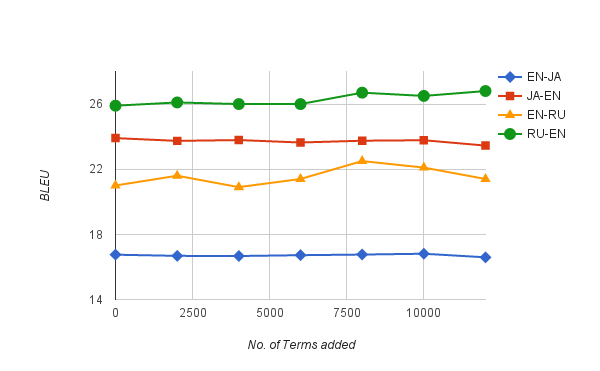
\includegraphics[width=17cm]{num-terms-in-mt.png} \\[-1em]
	\caption{Adding Automatically Extracted Terminology of Different Sizes to SMT}
	\label{fig-numterminmt}
\end{figure}


Table 3.5 and Figure 3.3. presents the results of passively adding varying numbers of  automatically extract bilingual terms to the training data before the statistical machine translation training process. From Table 3.5, we see that adding the top 10,000 bilingual terms to the English-Japanese data yields the highest BLEU score of 16.81 and its statistically significantly (p $<$ 0.05) better than  the baseline system without the added terminology. But this is not the case of the other direction; for Japanese-English, adding the automatically extracted bilingual terminology does not improve upon the baseline but it is also not statistically significantly worse than the baseline.

As for English to Russian, the added terminology performs best (BLEU=22.5) when 8,000 terms are added. In the reverse direction, the BLEU scores can be raised from 25.9 to 26.8 by adding the 12,000 extracted terms.

The results obtain confirms the previous work on adding lexical information to the training set in the attempt of improving machine translation. Most often, previous work as described in Chapter 2 (esp. Section 2.4.3), achieved marginal BLEU gains when passively adding additional lexical information to the training data in a non domain adaptation scenario where the terminology and corpus comes form the same domain.

\section{Summary}

In this chapter, we have proposed a novel information theoretic statistical term extraction technique based on a language model ($PMI_{LM}$) and we have intrinsically and extrinsically evaluated the quality of the terms extracted using the $PMI_{LM}$ based approach.

We show that the $PMI_{LM}$ provides state-of-art performance in extracting biomedical terms in both an unsupervised and a supervised scenario. We have also shown that given the optimal configuration of the automatically extracted terminology and passive integration of the term pairs in statistical machine translation, it is possible to achieve statistically significant though marginal BLEU score improvements.

In Chapter 4, we will describe more experiments to gain insights on how adding manually crafted and automatically extracted dictionary/terminology resource can improve phrased-based statistical machine translation. In the experiments reported in this chapter, ading automatically extracted lexicon passively provides statistically significant but marginal BLEU gains.   
